\documentclass[letterpaper]{article}

\date{Due: November 6, 11:59 pm}

\usepackage[margin=1in]{geometry}
% \usepackage{hyperref}
\usepackage[colorlinks]{hyperref}
\usepackage{capt-of}
\usepackage{amssymb}
\usepackage{amsmath}
\usepackage{url}
\usepackage{graphicx}
\usepackage{color}
\usepackage{bbm}
\usepackage{float}
\def\argmin{\mathop{\text{arg\,min}}}
\def\argmax{\mathop{\text{arg\,max}}}
\newcommand{\cov}{\mathrm{cov}}
\newcommand{\E}{\mathbb{E}}
\newcommand {\bX}{\mathbf{X}}
\newcommand {\bU}{\mathbf{U}}
\newcommand {\bS}{\mathbf{S}}
\newcommand {\bV}{\mathbf{V}}
\newcommand {\bH}{\mathbf{H}}
\newcommand{\mbf}[1]{{\mathbf{#1}}}
\usepackage{listings}
\usepackage{subcaption}

\def\argmin{\mathop{\text{arg\,min}}}
\def\argmax{\mathop{\text{arg\,max}}}

%\newcommand{\sol}{1}
%New colors defined below
\definecolor{codegreen}{rgb}{0,0.6,0}
\definecolor{codegray}{rgb}{0.5,0.5,0.5}
\definecolor{codepurple}{rgb}{0.58,0,0.82}
\definecolor{backcolour}{rgb}{0.95,0.95,0.92}

%Code listing style named "mystyle"
\lstdefinestyle{mystyle}{
	backgroundcolor=\color{backcolour},   commentstyle=\color{codegreen},
	keywordstyle=\color{magenta},
	numberstyle=\tiny\color{codegray},
	stringstyle=\color{codepurple},
	basicstyle=\footnotesize,
	breakatwhitespace=false,         
	breaklines=true,                 
	captionpos=b,                    
	keepspaces=true,                 
	numbers=left,                    
	numbersep=5pt,                  
	showspaces=false,                
	showstringspaces=false,
	showtabs=false,                  
	tabsize=2
}

\lstset{style=mystyle}

\newcommand{\Solution}[1]{{\color{blue} \paragraph{\bf $\bigstar $ SOLUTION:} { \sf
    #1} \bigskip}}
\begin{document}

{\centering
  \rule{6.3in}{2pt}
  \vspace{1em}
  {\Large
    CS589 Machine Learning - Fall 2020 \\
    Homework 5: CNN and Dimensionality Reduction \\
  }
  \vspace{1em}
  Due: November 6, 11:59 pm \\
  \vspace{0.1em}
  \rule{6.3in}{1.5pt}
}
\vspace{1pc}

%\maketitle

\paragraph*{Getting Started:} You should complete the assignment using your own installation of Python 3.6. Download the assignment archive from Moodle and unzip the file. This will create the directory structure as shown below. You will write your code under the Submission/Code directory. Make sure to put the deliverables (explained below) into the respective directories.

\begin{verbatim}
HW05
--- Data
    |-- Reduced MNIST Dataset
    |-- baboon.tiff
    Code
    |-- CNN_Template.py
    |-- svd_template.py
    |-- PCA_template.py
--- Submission
    |--Code
    |--Figures    
    |--Predictions
\end{verbatim}

If you are stuck on a question consider attending the office hours of the TA listed for that question.

\paragraph*{Data Sets:} For this homework, we'll use a subset of the MNIST dataset of handwritten digits containing 10 classes (digits 0-9). The first 100 digits (each 28x28 pixels) in the dataset are shown in the figure below.  \vspace{12pt}

\begin{table}[h!]
\center
\begin{tabular}{|l|c|c|c|c|}\hline
Dataset & Training Cases & Test Cases & Dimensionality & Target \\\hline\hline
Reduced MNIST Dataset & 10000 & 10000 & 784 & 10 Classes (0-9) \\\hline
\end{tabular}
\end{table}
\begin{center}
    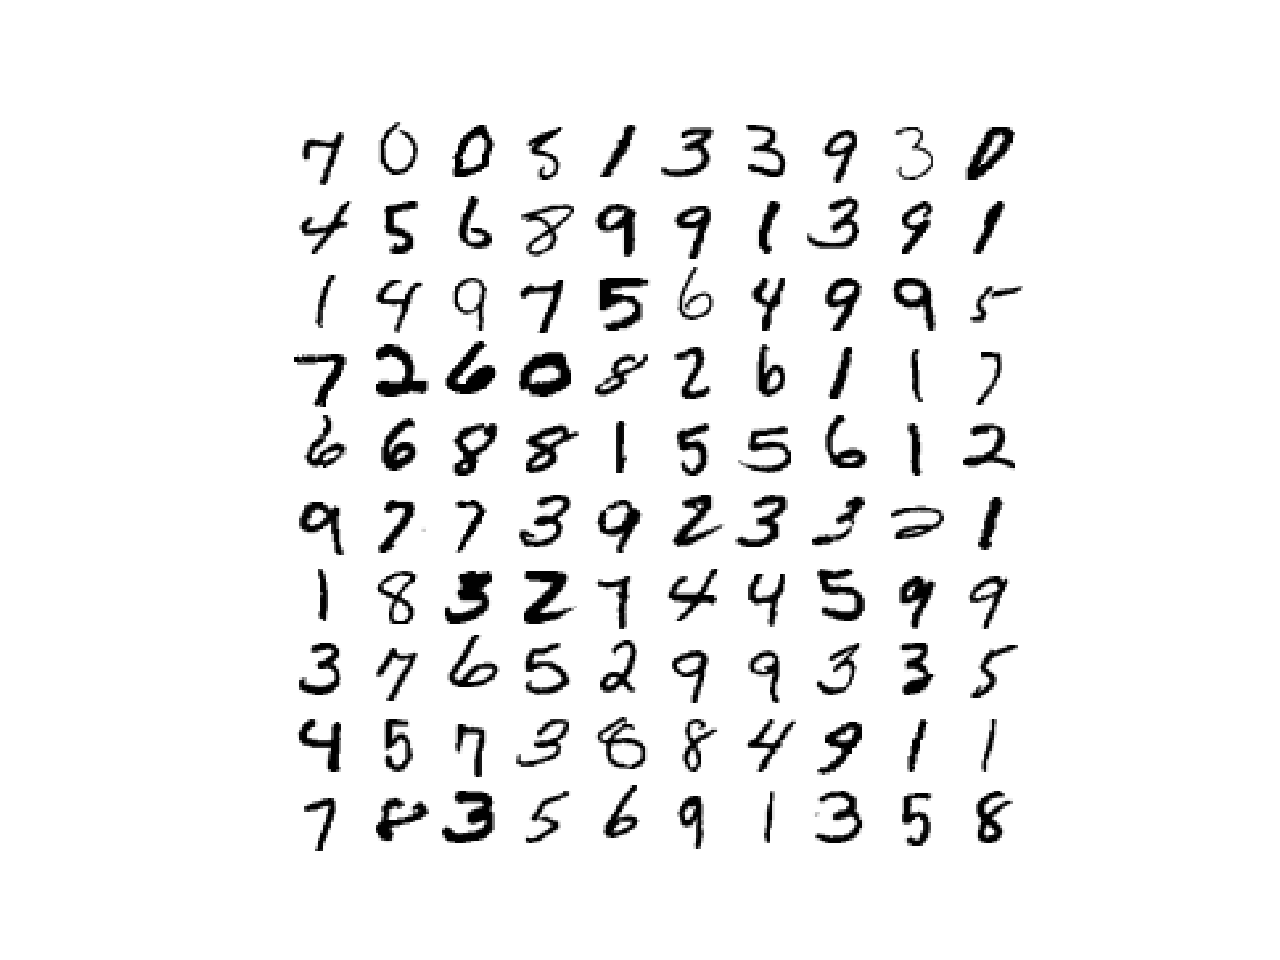
\includegraphics[scale=0.5]{mnist.png}
\end{center}

\paragraph*{Deliverables:} This assignment has three types of deliverables: a report, code files, and Kaggle submissions. 
\begin{itemize}
\item \textbf{Report: } The solution report will give your answers to the homework questions (listed below). The maximum length of the report is 5 pages in 11 point font, including all figures and tables. You can use any software to create your report, but your report must be submitted in PDF format. 

\item \textbf{Code: } The second deliverable is the code that you wrote to answer the questions, which will involve training classifiers and making predictions on held-out test data. Your code must be Python 3.6 (no iPython notebooks, other formats or code from other versions). You may create any additional source files to perform data analysis. However, you should aim to write your code so that it is possible to re-produce all of your experimental results exactly by running \textit{python run\_me.py} file from the Submissions/Code directory. Remember to comment your code. Points will be deducted from your assignment grade if your code is difficult to reproduce!

\end{itemize}

\paragraph*{Submitting Solutions:} When you complete the assignment, place your final code in Submission/Code and the Kaggle prediction files for your single best-performing submission in Submission/Predictions/best.csv. If you used Python to generate plots then place them in Submission/Figures. Finally, create a zip file called `Submission.zip' from your `Submission' directory only (do not include `Data' directory). Only .zip files will be accepted for grading code (not .tar, .rar, .gz, etc.). You will upload your .zip file of code and your pdf report to Gradescope for grading. Further instructions for using Gradescope will be provided on Piazza and discussed in class.

\paragraph*{Academic Honesty Statement:} Copying solutions from external sources (books, web pages, etc.) or other students is considered cheating. Sharing your solutions with other students is  considered cheating. Posting your code to public repositories like GitHub is also considered cheating. Any detected cheating will result in a grade of 0 on the assignment for all students involved, and potentially a grade of F in the course.

\paragraph*{Note:} You may use \underline{PyTorch} for the model implementations in all questions unless otherwise specified. \\

\section{Convolutional Neural Networks [40 points]}

\begin{enumerate}

\item {[10 points]} In order to see the advantage of convolutional neural networks over regular ones, lets compute the number of parameters for the following layer. Suppose, the input to the layer is a NxN dimensional feature which gets mapped to a NxNxC dimensional feature.
    \begin{enumerate}
    
    \item {[5 points]} How many parameters will a fully-connected layer have? Assume that we have a parameter for each connection from an input unit to an output unit.
    
    \item {[5 points]} Now assume we have C filters of size KxK, each of which is convolved with the input feature to produce a channel of the output feature. After suitable padding, the output of the convolution can be made equal to NxN dimensions. How many parameters does this layer have?
    
    \end{enumerate}
    
    \item {[30 points]} Now, implement a convolutional neural network for classifying MNIST digits using PyTorch and the provided template \texttt{CNN\_template.py}. In particular, you need to define your layers in the \texttt{\_\_init\_\_()} function, and define the connectivity between the layers in the \texttt{forward()} function of class \texttt{Convnet(nn.Module)}. Use the configuration provided in the table below. For training, use a batch size of 32, and the Adam optimizer (\texttt{torch.optim.Adam}) with learning rate of 0.01 and weight decay of 0.0001 for 10 epochs. You may use the training code that is included in the template. 

\begin{tabular}{|c|c|c|c|c|c|c|c|}
\hline
\textbf{Layer} & \textbf{Activation} & \textbf{\#Filters} & \textbf{Filter Size} & \textbf{Stride} & \textbf{Padding} & \textbf{o/p size} & \textbf{\#Params} \\ \hline
\multicolumn{8}{|c|}{Input (28 x 28)}                                                                                                                               \\ \hline
Conv2d         & ReLU                & 32                 & 3x3                  & 1               & 0                &                         &                   \\ \hline
Conv2d         & ReLU                & 64                 & 3x3                  & 1               & 0                &                         &                   \\ \hline
MaxPool2d      & -                   & -                  & 2x2                  & 2               & 0                &                         &                   \\ \hline
\multicolumn{6}{|c|}{Dropout2d (p=0.25)}                                                                              &                         &                   \\ \hline
\multicolumn{6}{|c|}{Flatten()}                                                                                       &                         &                   \\ \hline
Linear         & ReLU                & 128                & -                    & -               & -                &                         &                   \\ \hline
\multicolumn{6}{|c|}{Dropout (p=0.5)}                                                                                 &                         &                   \\ \hline
Linear         & Softmax             & 10                 & -                    & -               & -                &                         &                   \\ \hline
\end{tabular}

Now, answer the following questions:
\begin{enumerate}
    \item {[10 points]} Fill the columns for output size (dimensions of the output feature map) and number of parameters for each layer in the above table.
    
    \item {[10 points]} Plot the training and test accuracy with respect to number of epochs of training (10 epochs, LR=0.01, weight decay=0.0001).
    
    \item {[5 points]} What fraction of the total number of parameters is contained in the convolutional layers and fully connected layers? Explain if these results are surprising to you. 
    

\end{enumerate}

\end{enumerate}
\section{Singular Value Decomposition [40 points + 10 Extra Credit]}
Singular Value Decomposition\footnote{\url{http://en.wikipedia.org/wiki/Singular_value_decomposition}} is a powerful matrix decomposition with many applications. In a real world scenario one is interested in a low rank approximation of the matrix. 
Specifically, consider a matrix $\bX \in \mathbb{R}^{n \times m}$. 
According to the SVD theorem, $\bX$ can be expressed as:

\begin{equation}
\bX = \sum_{i=1}^r \sigma_i u_i v_i^T
\label{eq:svd1}
\end{equation} 
where $\sigma_1 \geq \sigma_2 \geq \ldots \geq \sigma_r$ are the singular 
values, $u_i \in \mathbb{R}^n$ for $i=1,\ldots,r$ are the left singular
vectors and $v_i \in \mathbb{R}^m$ for $i=1,\ldots,r$ are the right singular
vectors and $r$ is the rank of the matrix. 
Let $\bX_k$ be the $k-rank$ approximation of $\bX$:
\begin{equation}
\bX_k = \bU\bS\bV^T = \sum_{i=1}^k \sigma_i u_i v_i^T
\label{eq:svd2}
\end{equation} 
where $\bS$ is a $K \times K$ diagonal matrix with positive elements, $\bU$ is an $N \times K$ matrix such that $U^TU = I$, and $\bV$ is a $D \times K$ matrix such that $V^TV = I$. Typically, $k<<r$. Matrix $\bX_k$, the $k$-rank approximation of $\bX$ is optimal with respect to the 2 norm and the Frobenius norm.
For example: $|| \bX- \bX_k||_F \leq ||\bX-C||_F$ for any matrix $C$ of rank at most $k$ (including $k$). 
In this exercise you will implement a practical algorithm which comes with guarantees on its quality.

\paragraph{\textbf{Implementation:}}
In many cases we are willing to compute a sub-optimal $k$ rank approximation, $\hat{\bX}_k$ if we have important computational savings. You will implement an algorithm that finds $\hat{\bX}_k$ instead of $\bX_k$ and comes with guarantees on the quality of the approximation as already mentioned. This is done by calculating the approximation of the right singular matrix $\bV$.  The template for the implementation is in \texttt{Code/svd\_template.py}. 
The function you will write should have the following input and output arguments: 

\begin{itemize} 
\item Input 
	\begin{enumerate} 
		\item Matrix $X \in \mathbb{R}^{n \times m}$
		\item Integer $s \leq n$.
		\item Integer $k \leq s$.
\end{enumerate}
\item Output
		\begin{enumerate} 
		\item Matrix $\bH \in \mathbb{R}^{m \times k}$, which is the approximation to right singular matrix $\bV$
		\item $\lambda_1, \ldots, \lambda_k \in \mathbb{R}^+$.
		\end{enumerate}
\end{itemize} 

Matrix $H$ will contain the approximation to the top-$k$ right singular
vectors and $\lambda_1, \lambda_k$ is the approximation to the singular 
values.

\begin{enumerate}
\item \textbf{[25 points]} Implement the following algorithm:

\begin{enumerate} 
\item For $i = 1$ to $n$ compute $p_i = ||\bX(i,:)||^2/||\bX||^2_F$.
\item For $i = 1$ to $s$ 
      \begin{itemize} 
      \item Pick an integer $j$ from 1 to n with probability $Pr(\text{pick j})=p_j$.
      \item Include $\bX(j,:)$ as a row of S.
      \end{itemize}
\item Compute $S S^T$ and its singular value decomposition, i.e., $SS^T =\sum_{t=1}^s \lambda_t^2 w_t w_t^T$.
\item Compute $h_t =\frac{S^T w_t}{||S^T w_t||}$ for $t=1\ldots k$.
\item Return matrix $\bH$ whose columns are the vectors $h_1,\ldots,h_k$ and $\lambda_1 \geq \ldots \geq \lambda_k$. 
\end{enumerate}

You are allowed to use following functions to implement below algorithm. 
\begin{enumerate}
    \item \texttt{np.linalg.norm}: To calculate the frobenius norm of the matrix $||\bX||_F$.
    \item \texttt{np.linalg.svd}: To calculate SVD of the matrix $SS^T$
    \item \texttt{np.random.choice}: To randomly choose index $j$ with probability $p_j$. 
\end{enumerate}

\textbf{Instruction:} As solution to this part, you need to provide your code \textit{only} for \texttt{SVD} function in the \textbf{report} since it should not be more than one page. Refer latex code provided with Homework to see how to use \textit{listings} package to include your python code in latex..

\lstinputlisting[language=Python]{Onlysvd_template_latex.py}
\item \textbf{[10 points Extra Credit]} The matrix $\hat{\bX}_k$ can be calculated from $H$ as follows:
$$\hat{\bX}_k = \bX\bH\bH^T$$


Explain why this is the case.

\textit{Hint:}  $\bH$ is the approximation of right singular matrix $\bV$. 


\item \textbf{[15 points]}
Apply your implementation to the image in \texttt{Data/baboon.tiff} image for $k = 60$ and $s = 80$ and compare to the optimal $60$-rank approximation.


\begin{enumerate}
\item  Plot the original image $\bX$ and two reconstructed images optimal k-rank approximation $\bX_k$ and sub-optimal k-rank approximation $\hat{\bX}_k$ using $\bH$ as indicated in the previous question.

\item Report the error in terms of the Frobenius norm for both the optimal 60 rank produced from the SVD and for the 60 rank approximation produced by your implementation. 
\end{enumerate}


\end{enumerate}

\section{Principle Component Analysis [20 points]}
In this part, you will be working on the MNIST dataset again (given in Data/X\_train.npy and Data/Y\_train.npy) and you will implement the PCA algorithm from scratch. The template for the implementation is in \texttt{Code/PCA\_template.py}

\begin{enumerate}

	\item {\textbf{[5 points]}} Use PCA to get a new set of bases. You are required to implement the PCA algorithm. You are allowed to use library functions for eigenvalue decomposition and covariate matrix, in Python \texttt{np.linalg.eig and np.cov} will do the trick. Plot the eigenvalues in descending order (eigenvalues at y-axis) and report how many components you would pick from the plot and explain why.
	
	\item {\textbf{[5 points]}} Display the sample mean of the dataset as an image. Also display the sample mean images for each digit (use subfigure in matplotlib to plot all of these). Add all images to your report.
	\item {\textbf{[5 points]}} Display the top 5 eigenvectors as images and add them to your report. Interpret these images, which number(s) do they look like, what is captured by these eigenvectors?

	\item {\textbf{[5 points]}} Project your dataset on the first and second principal components and plot this projection (you may want to use a scatter plot), using a different color for each digit. Describe the plot, from the perspective of digit similarity. Which groups of digits are close to each other?
	
\end{enumerate}

\end{document}

